\section{Træer}
\subsection{Terminologi for træer}

\begin{defn}
Et træ er en sammenhængende ikke-orienteret graf, der ikke indeholder en simpel kreds.
\label{def_tree}
\end{defn}

\noindent Træer er en type af simple grafer, da de ikke indeholder en simpel kreds. Derfor kan der ikke være flere kanter mellem to knuder, og der kan ikke være løkker. Alternativt og ekvivalent til Definition \ref{def_tree} kan et træ defineres som følger.

\begin{thm}
En ikke-orienteret graf er et træ hvis og kun hvis, der eksistrerer netop én simpel vej mellem hvert par af knuder. 
\end{thm}

\begin{proof}
Antag at en ikke-orienteret graf $T$ er et træ, og lad $u$ og $v$ være to knuder i $T$. Da $T$ er sammenhængende må det betyde, at der er en simpel vej mellem $u$ og $v$ jf. Sætning \ref{smh_satning}. Den simple vej mellem $u$ og $v$ må være den eneste vej mellem $u$ og $v$, for hvis der eksisterer flere veje mellem $u$ og $v$, dannes en simpel kreds. Eksistensen af en simpel kreds modstrider antagelsen om, at $T$ er et træ, og derfor må der være netop én simpel vej mellem hvert knudepar i $T$.

Antag nu, at der er netop én simpel vej mellem hvert knudepar i en ikke-orienteret graf $T$. Det betyder, at $T$ er sammenhængende. Desuden må det gælde, at $T$ ingen kredse har, da det vil stride i mod antagelsen om, at der er netop én simpel vej mellem hvert knudepar i en $T$. Grafen $T$ opfylder dermed kravene for at være et træ jf. Definition \ref{def_tree}, og da $T$ er en ikke-orienteret graf med netop én simpel vej mellem hvert knudepar, kan et træ defineres på denne måde.
\end{proof}

\begin{exmp}
For at illustrere en graf, som er et træ, og en graf, som ikke et træ, iagttages hhv. Figur \ref{eksempel_tree} og Figur \ref{eksempel_notree}. Grafen i Figur \ref{eksempel_tree} er et træ, da det er en ikke-orienteret sammenhængende graf uden simple kredse.
\end{exmp}

\begin{figure}[h]
\centering
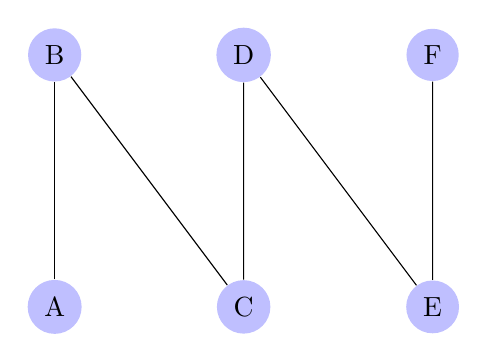
\begin{tikzpicture}
[scale=.8,auto=left,every node/.style={circle,fill=blue!25}]
  \node (n6) at (3,2) {A};
  \node (n4) at (3,6) {B};
  \node (n5) at (6,2) {C};
  \node (n1) at (6,6) {D};
  \node (n2) at (9,2) {E};
  \node (n3) at (9,6) {F};
  \foreach \from/\to in {n6/n4,n4/n5,n5/n1,n1/n2,n2/n3}
    \draw (\from) -- (\to);
\end{tikzpicture}
\caption{Et træ.} 
\label{eksempel_tree}
\end{figure}

\noindent Grafen i Figur \ref{eksempel_notree} er ikke et træ, da der eksistrer en kreds $\lbrace B, D, E \rbrace$. Grafen er heller ikke et træ med argumentet, at grafen ikke er sammenhængende.\\

\begin{figure}[h]
\centering
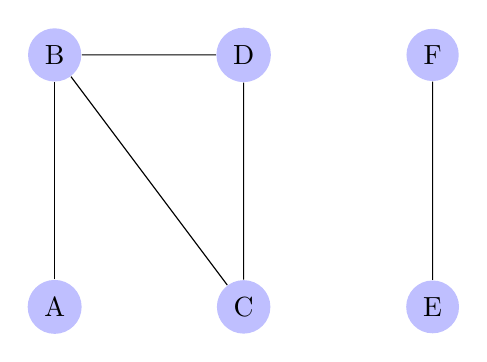
\begin{tikzpicture}
[scale=.8,auto=left,every node/.style={circle,fill=blue!25}]
  \node (n6) at (3,2) {A};
  \node (n4) at (3,6) {B};
  \node (n5) at (6,2) {C};
  \node (n1) at (6,6) {D};
  \node (n2) at (9,2) {E};
  \node (n3) at (9,6) {F};
  \foreach \from/\to in {n6/n4,n4/n5,n5/n1,n2/n3,n4/n1}
    \draw (\from) -- (\to);
\end{tikzpicture}
\caption{En graf, der ikke er et træ.} 
\label{eksempel_notree}
\end{figure}

\noindent Mange anvendelser af træer, kræver at en bestemt knude i en graf fungerer som udgangspunkt. En knude kan indentificeres som en rod, og dermed rodfæste grafen.

\begin{defn}
Et rodfæstet træ er et træ med en knude, der er dedikeret som roden. De resterende knuder er orienteret væk fra roden.
\end{defn}

\noindent Der findes terminologi, der beskriver knudernes forhold til hinanden i en rodfæstet graf. 
Hvis $T$ er et rodfæstet træ, så er en knude $v$, som ikke er roden, $\textit{forælder}$ til en knude $u$, hvis der eksiterer en orienteret kant mellem $v$ og $u$ i retningen væk fra roden.
Samtidigt er $u$ $\textit{barn}$ af $v$, og knuder med samme forælder kaldes $\textit{søskende}$. 
$\textit{Forfædrene}$ til $v$ er knuderne på vejen fra roden til $v$, og $\textit{efterkommerne}$ til $v$ er knuderne, der har $v$ som forfader. 
Knuder, der har børn kaldes $\textit{indre knuder}$, og knuder, der ikke har børn kaldes $\textit{blade}$.
Hvis $w$ er en knude i et træ, så er et undertræ med $w$ som rod, træet, det består af $w$ og alle dets efterkommere og alle kanter incidente til efterkommerne.

\begin{exmp}
Betragt træet i Figur \ref{eksempel_rootedtree}. 
For at eksemplificere terminologien, så er roden af træet $a$, og $a$ er forælder til $b$ og $c$, hvilket vil sige, at $b$ og $c$ er børn til $a$, og $b$ og $c$ er hinandens søskende. 
Knuden $b$ er efterkommer af $a$, og den er forfader til $\lbrace d, e, f \rbrace$. 
I grafen er $a$, $b$ og $c$ grafens indre knuder, og mængden af blade er $\lbrace d, e, f, g, h, i \rbrace$. 
Et eksempel på en undertræ af træet i Figur \ref{eksempel_rootedtree} er træet i Figur \ref{eksempel_rootedsubtree}.
Undertræet har $b$ som rod og indeholder efterkommerne af $b$ og kanterne incidente med dem. 
\end{exmp}

\begin{figure}[h]
\centering
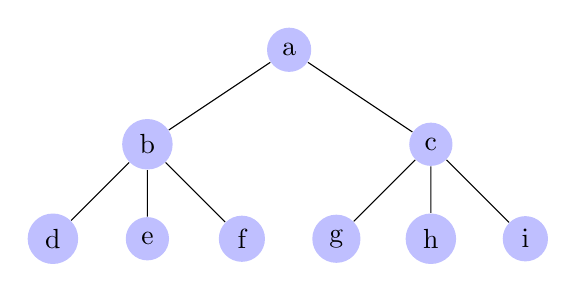
\begin{tikzpicture}
[scale=.8,auto=left,every node/.style={circle,fill=blue!25}]
  \node {a}
  	child{node{b}
  		child{node{d}}
  		child{node{e}}
  		child{node{f}}}
  	child[missing]
  	child[missing]
  	child{node{c}
  		child{node{g}}
  		child{node{h}}
  		child{node{i}}};
\end{tikzpicture}
\caption{Et rodfæstet træ.} 
\label{eksempel_rootedtree}
\end{figure}

\begin{figure}[h]
\centering
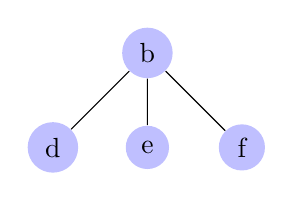
\begin{tikzpicture}
[scale=.8,auto=left,every node/.style={circle,fill=blue!25}]
  \node {b}
  	child{node{d}}
  	child{node{e}}
  	child{node{f}};
\end{tikzpicture}
\caption{Et undertræ med $b$ som rod.} 
\label{eksempel_rootedsubtree}
\end{figure}

\subsection{Udspændende træer}
